\documentclass[border=1pt]{standalone}
\usepackage[T1]{fontenc}
\usepackage{newtxtext,newtxmath}
\usepackage{amsmath}
\usepackage{tikz}
\usetikzlibrary{arrows.meta,positioning,fit}

\begin{document}
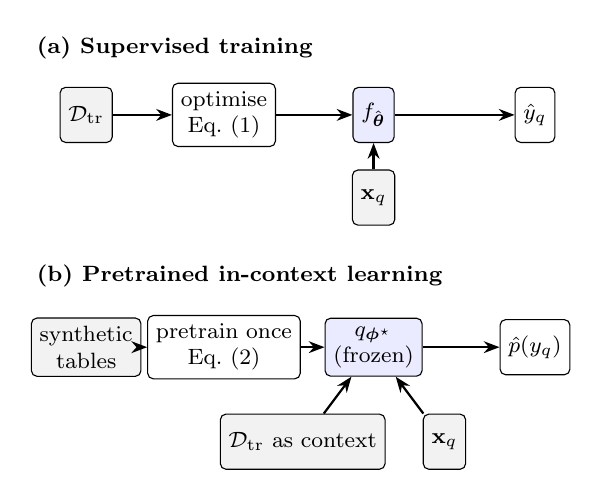
\begin{tikzpicture}[
  font=\footnotesize,
  box/.style={draw, rounded corners=2pt, align=center, minimum height=7mm, inner sep=3pt},
  data/.style={box, fill=gray!10},
  model/.style={box, fill=blue!8},
  arrow/.style={-{Stealth[length=2mm]}, thick}]
\node[font=\footnotesize\bfseries, anchor=west] at (-0.15,0.85) {(a) Supervised training};
\node[data] (tr) at (0.6,0) {$\mathcal{D}_{\mathrm{tr}}$};
\node[box] (fit) at (2.35,0) {optimise\\Eq.~(1)};
\node[model] (theta) at (4.25,0) {$f_{\hat{\boldsymbol\theta}}$};
\node[data] (xq1) at (4.25,-1.05) {$\mathbf{x}_q$};
\node[box] (y1) at (6.3,0) {$\hat{y}_q$};
\draw[arrow] (tr) -- (fit); \draw[arrow] (fit) -- (theta); \draw[arrow] (theta) -- (y1);
\draw[arrow] (xq1) -- (theta);
\node[font=\footnotesize\bfseries, anchor=west] at (-0.15,-2.05) {(b) Pretrained in-context learning};
\node[data] (syn) at (0.6,-2.95) {synthetic\\tables};
\node[box] (pre) at (2.35,-2.95) {pretrain once\\Eq.~(2)};
\node[model] (phi) at (4.25,-2.95) {$q_{\boldsymbol\phi^{\star}}$\\(frozen)};
\node[data] (ctx) at (3.35,-4.15) {$\mathcal{D}_{\mathrm{tr}}$ as context};
\node[data] (xq2) at (5.15,-4.15) {$\mathbf{x}_q$};
\node[box] (y2) at (6.3,-2.95) {$\hat{p}(y_q)$};
\draw[arrow] (syn) -- (pre); \draw[arrow] (pre) -- (phi); \draw[arrow] (phi) -- (y2);
\draw[arrow] (ctx) -- (phi); \draw[arrow] (xq2) -- (phi);
\end{tikzpicture}
\end{document}
